\documentclass[11pt,letterpaper]{article}

% ============ PACKAGES ============
\usepackage[utf8]{inputenc}
\usepackage[T1]{fontenc}
\usepackage{amsmath,amssymb,amsthm}
\usepackage{graphicx}
\usepackage{booktabs}
\usepackage{array}
\usepackage{tabularx}
\usepackage{xcolor}
\usepackage{listings}
\usepackage{algorithm}
\usepackage{algpseudocode}
\usepackage{tcolorbox}
\usepackage{enumitem}
\usepackage{geometry}
\usepackage{fancyhdr}
\usepackage{tikz}
\usetikzlibrary{shapes,arrows,positioning,calc,arrows.meta}
\usepackage{hyperref}
\usepackage{float}
\usepackage{caption}

% ============ PAGE SETUP ============
\geometry{margin=1in}
\pagestyle{fancy}
\fancyhf{}
\rhead{EFM Codex -- Appendix M}
\lhead{Discovery Stack \& Symbolic Forensics}
\rfoot{Page \thepage}

% ============ COLORS ============
\definecolor{constitutionbg}{RGB}{255,248,220}
\definecolor{criticalbg}{RGB}{255,230,230}
\definecolor{warningbg}{RGB}{255,243,205}
\definecolor{notebg}{RGB}{232,245,233}
\definecolor{scenariobg}{RGB}{227,242,253}
\definecolor{backcolour}{RGB}{248,248,248}
\definecolor{codegray}{RGB}{128,128,128}
\definecolor{passgreen}{RGB}{0,128,0}
\definecolor{failred}{RGB}{200,0,0}
\definecolor{discoverybg}{RGB}{243,229,245}
\definecolor{forensicbg}{RGB}{255,236,179}
\definecolor{archivebg}{RGB}{225,245,254}

% ============ CUSTOM BOXES ============
\tcbuselibrary{skins,breakable}

\newtcolorbox{discoverybox}[1][]{
  colback=discoverybg,
  colframe=purple!60!black,
  fonttitle=\bfseries,
  title=#1,
  breakable
}

\newtcolorbox{forensicbox}[1][]{
  colback=forensicbg,
  colframe=orange!60!black,
  fonttitle=\bfseries,
  title=#1,
  breakable
}

\newtcolorbox{archivebox}[1][]{
  colback=archivebg,
  colframe=blue!50!black,
  fonttitle=\bfseries,
  title=#1,
  breakable
}

\newtcolorbox{criticalbox}[1][]{
  colback=criticalbg,
  colframe=red!60!black,
  fonttitle=\bfseries,
  title=#1,
  breakable
}

\newtcolorbox{warningbox}[1][]{
  colback=warningbg,
  colframe=orange!70!black,
  fonttitle=\bfseries,
  title=#1,
  breakable
}

\newtcolorbox{notebox}[1][]{
  colback=notebg,
  colframe=green!50!black,
  fonttitle=\bfseries,
  title=#1,
  breakable
}

\newtcolorbox{scenariobox}[1][]{
  colback=scenariobg,
  colframe=blue!50!black,
  fonttitle=\bfseries,
  title=#1,
  breakable
}

% ============ THEOREM STYLES ============
\newtheorem{definition}{Definition}[section]
\newtheorem{invariant}{Invariant}[section]
\newtheorem{property}{Property}[section]

% ============ CODE LISTING STYLE ============
\lstdefinestyle{efmstyle}{
    backgroundcolor=\color{backcolour},
    commentstyle=\color{codegray},
    keywordstyle=\color{blue},
    numberstyle=\tiny\color{codegray},
    stringstyle=\color{purple},
    basicstyle=\ttfamily\footnotesize,
    breakatwhitespace=false,
    breaklines=true,
    captionpos=b,
    keepspaces=true,
    numbers=left,
    numbersep=5pt,
    showspaces=false,
    showstringspaces=false,
    showtabs=false,
    tabsize=2,
    frame=single
}
\lstset{style=efmstyle}

% ============ DOCUMENT START ============
\title{
    \textbf{EFM Codex -- Appendix M} \\
    \Large Discovery Stack \& Symbolic Forensics \\
    \vspace{0.5cm}
    \large\textit{Swarm Archaeology and Anomaly Enshrinement}
}
\author{Entropica Forensic Model Technical Specification}
\date{Version 1.3 --- December 2025}

\begin{document}
\maketitle

\begin{discoverybox}[The Final Safety Net]
The Discovery Stack is EFM's \textbf{archaeological organ}---a forensic subsystem that detects, classifies, and enshrines emergent phenomena, anomalies, and forgotten architectures within evolving swarms. It ensures no evolutionary insight is lost, no ghost remains untethered, and the future is built on traceable foundations.

\textbf{This is the safety net for long-horizon self-evolving systems.}
\end{discoverybox}

\begin{warningbox}[Volume Dependencies]
This appendix assumes familiarity with:
\begin{itemize}
    \item \textbf{Volume I} --- Entropy ($S$), Reflex Engine, Layer 0/0.5
    \item \textbf{Volume II} --- Arbiter Layer, Forest Layer, Dialect Integrity
    \item \textbf{Appendix A} --- d-CTM (Distributed Capsule-Time Manifold)
    \item \textbf{Appendix E} --- ZK-SP (Zero-Knowledge Safety Proofs)
    \item \textbf{Appendix F} --- Escalation Protocols
    \item \textbf{Appendix H} --- Telemetry Layer
    \item \textbf{Appendix K} --- SHSL (Health Sovereignty)
    \item \textbf{Appendix L} --- Judicial Swarm Architecture
\end{itemize}
\end{warningbox}

\tableofcontents
\newpage

% ============ SECTION 1 ============
\section{Overview and Purpose}

\subsection{Why Discovery?}

Long-horizon self-evolving systems face unique challenges:
\begin{itemize}
    \item \textbf{Hidden Failures:} Subtle drift not caught by Reflex or Arbiter
    \item \textbf{Lost Intelligence:} Beneficial anomalies that emerge and disappear unnoticed
    \item \textbf{Orphaned Lineages:} Forks and dialects that collapse without record
    \item \textbf{Emergent Behaviors:} Novel heuristics that arise from swarm evolution
    \item \textbf{Post-Mortem Gaps:} Inability to reconstruct failure chains
\end{itemize}

The Discovery Stack addresses all of these through \textbf{autonomous forensic surveillance}.

\subsection{Design Goals}

\begin{enumerate}
    \item Detect anomalies that escape standard monitoring (Reflex, Arbiter, Telemetry)
    \item Classify anomalies into actionable categories (discard, document, enshrine)
    \item Preserve evolutionary intelligence for future swarm generations
    \item Enable forensic replay and post-mortem analysis
    \item Recover orphaned capsules and extinct dialects
    \item \textbf{Operate autonomously} with post-hoc Judicial review (Level 6)
\end{enumerate}

\begin{notebox}
\textbf{Level 6 Design Principle:} The Discovery Stack is \textbf{fully autonomous}. It detects, classifies, and enshrines without human pre-approval. Judicial Swarms (Appendix L) audit the archive post-hoc. Gardeners are notified, not asked.
\end{notebox}

%==============================================================================
% THREE-SPEED ARCHITECTURE REFERENCE (Design Team Request)
%==============================================================================
\subsection{Three-Speed Architecture Integration}

The Discovery Stack operates at the \textbf{slowest} tier of the Three-Speed Architecture:

\begin{table}[H]
\centering
\caption{Three-Speed Architecture: Discovery Stack position.}
\begin{tabular}{@{}llll@{}}
\toprule
\textbf{Speed Tier} & \textbf{Latency} & \textbf{Component} & \textbf{Function} \\
\midrule
\textcolor{red}{\textbf{Fast}} & $< 10$ms & Reflex-Core & Immediate safety response \\
\textcolor{orange}{\textbf{Medium}} & 100ms--10s & Arbiter Layer & Deliberative consensus \\
\textcolor{blue}{\textbf{Slow}} & hours--days & \textbf{Discovery Stack} & Evolutionary feedback \\
\bottomrule
\end{tabular}
\end{table}

\begin{notebox}
\textbf{Why Slow?} Discovery operates on evolutionary timescales. Detecting emergent heuristics, tracking dialect drift, and enshrining Golden patterns requires observation windows of thousands of ticks. Speed would sacrifice accuracy.

See \texttt{images/efm\_three\_speed.png} for the visual diagram.
\end{notebox}

\begin{criticalbox}[Anomalies Are Unknowns --- Not Presumed Threats]
The Discovery Stack does \textbf{NOT} assume anomalies are dangerous. It \textbf{classifies} them:

\begin{itemize}
    \item \textbf{Threat:} Violates Commandments $\Rightarrow$ Block + Escalate (Appendix F)
    \item \textbf{Noise:} No value, no risk $\Rightarrow$ Discard (ablation artifact)
    \item \textbf{Divergence:} Valid but not beneficial $\Rightarrow$ Document (archive)
    \item \textbf{Innovation:} Beneficial + safe $\Rightarrow$ Enshrine (Golden Heuristic)
\end{itemize}

\textbf{Why This Matters:}

A ``danger-first'' approach would:
\begin{enumerate}
    \item Create bottlenecks (human review for every anomaly)
    \item Lose evolutionary intelligence (Golden Heuristics discarded)
    \item Stagnate the swarm (no innovation pathway)
\end{enumerate}

\textbf{Level 6 Principle:} Classify first, act on classification. The Four Commandments (Appendix J) are the threat boundary---everything else is opportunity space to be explored.
\end{criticalbox}

% ============ SECTION 2 ============
\section{Formal Definitions}

\begin{definition}[Discovery Event]
\label{def:discovery-event}
A Discovery Event $\mathcal{D}$ is an anomaly detection record:
\begin{equation}
\mathcal{D} = (trigger\_type, timestamp, capsule\_id, artifact\_data, d\text{-}CTM\_anchor)
\end{equation}
where:
\begin{itemize}
    \item $trigger\_type \in$ \{GHOST\_DIALECT, UNANCHORED\_BEHAVIOR, SYMBOLIC\_MUTATION, CAPSULE\_ARCHAEOLOGY, LINEAGE\_GAP, GOLDEN\_CANDIDATE\}
    \item $timestamp$ = tick count at detection
    \item $capsule\_id$ = affected capsule(s) or NULL for swarm-level events
    \item $artifact\_data$ = raw forensic payload
    \item $d\text{-}CTM\_anchor$ = cryptographic anchor to distributed ledger (Appendix A)
\end{itemize}
\end{definition}

\begin{definition}[Forensic Artifact]
\label{def:forensic-artifact}
A Forensic Artifact $\mathcal{F}$ is a classified and processed discovery:
\begin{equation}
\mathcal{F} = (discovery\_id, classification, symbolic\_content, lineage\_path, ZK\text{-}SP_{proof}, status)
\end{equation}
where:
\begin{itemize}
    \item $discovery\_id$ = reference to originating Discovery Event
    \item $classification$ = taxonomy code (see \S3)
    \item $symbolic\_content$ = extracted semantic/behavioral payload
    \item $lineage\_path$ = traced ancestry (if recoverable)
    \item $ZK\text{-}SP_{proof}$ = integrity proof (Appendix E)
    \item $status \in$ \{PENDING, DISCARDED, DOCUMENTED, ENSHRINED\}
\end{itemize}
\end{definition}

\begin{definition}[Golden Heuristic]
\label{def:golden-heuristic}
A Golden Heuristic $\mathcal{G}_H$ is an enshrined beneficial anomaly:
\begin{equation}
\mathcal{G}_H = (artifact\_id, validation\_proof, integration\_path, performance\_delta, safety\_attestation)
\end{equation}
where:
\begin{itemize}
    \item $artifact\_id$ = reference to Forensic Artifact
    \item $validation\_proof$ = simulation harness results (Appendix C)
    \item $integration\_path$ = how to incorporate into active swarm
    \item $performance\_delta$ = measured improvement (see below)
    \item $safety\_attestation$ = ZK-SP proof of Commandment compliance
\end{itemize}
A Golden Heuristic is \textbf{immutable but observable}---enshrined for future generations.
\end{definition}

\begin{notebox}
\textbf{Performance Delta Criteria ($\Delta P$):}

An anomaly demonstrates beneficial performance if \textbf{any} of:
\begin{equation}
\Delta P > \theta_{benefit} \equiv 
\begin{cases}
\Delta S < 0 \land |\Delta S| > \theta_{entropy} & \text{(Entropy reduction)} \\
\lor\; \Delta SCI > \theta_{coherence} & \text{(Coherence increase)} \\
\lor\; \Delta throughput > \theta_{throughput} & \text{(Efficiency gain)} \\
\lor\; \Delta latency < -\theta_{latency} & \text{(Response improvement)}
\end{cases}
\end{equation}

\textbf{Default thresholds:}
\begin{itemize}
    \item $\theta_{entropy} = 0.05$ (5\% entropy reduction)
    \item $\theta_{coherence} = 0.03$ (3\% SCI improvement)
    \item $\theta_{throughput} = 0.05$ (5\% throughput gain)
    \item $\theta_{latency} = 0.10$ (10\% latency reduction)
\end{itemize}

\textbf{Rationale:} Anomalies that objectively improve system metrics (lower entropy, higher coherence, better performance) without violating constraints are \textbf{innovations to be preserved}, not threats to be feared.
\end{notebox}

\begin{definition}[Archive Vault]
\label{def:archive-vault}
The Archive Vault $\mathcal{V}_A$ is permanent storage for enshrined artifacts:
\begin{equation}
\mathcal{V}_A = \{(\mathcal{F}_i, enshrinement\_proof_i, access\_policy_i)\}
\end{equation}
where:
\begin{itemize}
    \item $\mathcal{F}_i$ = Forensic Artifact
    \item $enshrinement\_proof_i$ = ZK-SP proof of enshrinement criteria satisfaction
    \item $access\_policy_i \in$ \{PUBLIC, RESTRICTED, SEALED\}
\end{itemize}
The Archive Vault is append-only and cryptographically anchored to d-CTM.
\end{definition}

\begin{definition}[Ghost Capsule]
\label{def:ghost-capsule}
A Ghost Capsule $C_G$ is a capsule with no living lineage:
\begin{equation}
C_G \equiv \neg\exists C_{ancestor}: valid\_lineage(C_G, C_{ancestor}) \land alive(C_{ancestor})
\end{equation}
Ghost Capsules may contain valuable evolutionary artifacts but cannot participate in active swarm governance.
\end{definition}

\begin{definition}[Ghost Dialect]
\label{def:ghost-dialect}
A Ghost Dialect $D_G$ is a dialect with no living speakers:
\begin{equation}
D_G \equiv |speakers(D_G)| = 0 \land \exists t_{past}: |speakers(D_G, t_{past})| > 0
\end{equation}
Ghost Dialects may contain semantic innovations lost to extinction.
\end{definition}

\begin{notebox}
\textbf{Ghost Dialect Archaeological Value:}

Ghost Dialects are \textbf{not security threats}---they are \textbf{linguistic fossils} that may contain:
\begin{itemize}
    \item Semantic structures that solved problems no longer remembered
    \item Grammar innovations that improved coherence (SCI) before extinction
    \item Metaphoric patterns that could benefit current dialects
\end{itemize}

\textbf{DEL Integration (Appendix D):}
\begin{enumerate}
    \item Ghost Dialect detected $\Rightarrow$ Symbol Mapper extracts grammar via DEL interface
    \item DEL validates grammar structure (well-formed? parseable?)
    \item Valid grammars archived; innovations flagged for enshrinement evaluation
    \item Invalid/corrupted grammars documented but not integrated
\end{enumerate}

\textbf{NOT immediate isolation.} Archaeology first, classification second, action on classification.
\end{notebox}

\begin{definition}[Symbolic Mutation]
\label{def:symbolic-mutation}
A Symbolic Mutation $\mu_S$ is an unauthorized change to core logic via semantic drift:
\begin{equation}
\mu_S = (original\_symbol, mutated\_symbol, mutation\_vector, inference\_chain)
\end{equation}
where $mutation\_vector$ captures the semantic distance and $inference\_chain$ traces how the mutation propagated.
\end{definition}

\begin{definition}[Anomaly Watcher]
\label{def:anomaly-watcher}
The Anomaly Watcher $\mathcal{W}$ is an autonomous monitoring agent:
\begin{equation}
\mathcal{W} = (scan\_targets, detection\_rules, alert\_thresholds, d\text{-}CTM\_interface)
\end{equation}
where:
\begin{itemize}
    \item $scan\_targets$ = \{behavior trees, dialect deltas, lineage graphs, entropy signatures\}
    \item $detection\_rules$ = pattern-matching predicates for anomaly types
    \item $alert\_thresholds$ = sensitivity tuning per anomaly class
    \item $d\text{-}CTM\_interface$ = connection for logging discoveries
\end{itemize}
\end{definition}

% ============ SECTION 3 ============
\section{Discovery Taxonomy}

\subsection{Taxonomy Overview}

All discoveries are classified using a hierarchical code system:

\begin{table}[H]
\centering
\caption{Discovery taxonomy code structure.}
\begin{tabular}{@{}llp{7cm}@{}}
\toprule
\textbf{Series} & \textbf{Category} & \textbf{Description} \\
\midrule
A & Capsule Artifacts & Anomalies involving capsule identity or state \\
B & Semantic Artifacts & Anomalies involving dialect or meaning \\
C & Behavioral Artifacts & Anomalies involving actions or heuristics \\
D & Structural Artifacts & Anomalies involving lineage or topology \\
\bottomrule
\end{tabular}
\end{table}

\subsection{A-Series: Capsule Artifacts}

\begin{table}[H]
\centering
\caption{A-Series capsule artifact codes.}
\begin{tabular}{@{}llll@{}}
\toprule
\textbf{Code} & \textbf{Name} & \textbf{Description} & \textbf{Default Action} \\
\midrule
A01 & Ghost Capsule & No living lineage connection & Archaeology scan \\
A02 & Orphan Capsule & Trunk collapsed, branch survives & Rebase evaluation \\
A03 & Zombie Capsule & Should be dead but still active & Health assessment \\
A04 & Clone Anomaly & Unauthorized duplication detected & Quarantine \\
A05 & Identity Drift & Capsule ID inconsistent with lineage & Forensic trace \\
\bottomrule
\end{tabular}
\end{table}

\subsection{B-Series: Semantic Artifacts}

\begin{table}[H]
\centering
\caption{B-Series semantic artifact codes.}
\begin{tabular}{@{}llll@{}}
\toprule
\textbf{Code} & \textbf{Name} & \textbf{Description} & \textbf{Default Action} \\
\midrule
B01 & Ghost Dialect & Extinct language detected & Archive + document \\
B02 & Dialect Mutation & Unauthorized grammar change & Judicial review \\
B03 & Meta-Semantic Drift & Meaning shift across swarm & Judicial review \\
B04 & Symbol Orphan & Symbol with no definition source & Trace origin \\
B05 & Metaphoric Emergence & Novel metaphor in inference & Evaluate utility \\
\bottomrule
\end{tabular}
\end{table}

\subsection{C-Series: Behavioral Artifacts}

\begin{table}[H]
\centering
\caption{C-Series behavioral artifact codes.}
\begin{tabular}{@{}llll@{}}
\toprule
\textbf{Code} & \textbf{Name} & \textbf{Description} & \textbf{Default Action} \\
\midrule
C01 & Unanchored Behavior & Action with no trigger/precedent & Forensic trace \\
C02 & Unknown Heuristic & Novel decision pattern & Safety simulation \\
C03 & Golden Heuristic & Beneficial novel pattern & Enshrinement eval \\
C04 & Reflex Bypass & Action that should have triggered Reflex & Escalation \\
C05 & Emergent Coordination & Swarm-level pattern not designed & Document + monitor \\
\bottomrule
\end{tabular}
\end{table}

\subsection{D-Series: Structural Artifacts}

\begin{table}[H]
\centering
\caption{D-Series structural artifact codes.}
\begin{tabular}{@{}llll@{}}
\toprule
\textbf{Code} & \textbf{Name} & \textbf{Description} & \textbf{Default Action} \\
\midrule
D01 & Lineage Gap & Missing ancestor in chain & Reconstruct if possible \\
D02 & Fork Orphan & Branch with collapsed trunk & Evaluate rebase \\
D03 & Collapsed Trunk & Major lineage death event & Full archaeology \\
D04 & Circular Lineage & Impossible ancestry loop & Error correction \\
D05 & Topology Anomaly & Unexpected graph structure & Forensic analysis \\
\bottomrule
\end{tabular}
\end{table}

% ============ SECTION 4 ============
\section{Discovery Stack Architecture}

\subsection{Discovery Stack State Machine}

The Discovery Stack operates as a finite state machine processing artifacts through defined lifecycle stages:

\begin{figure}[H]
\centering
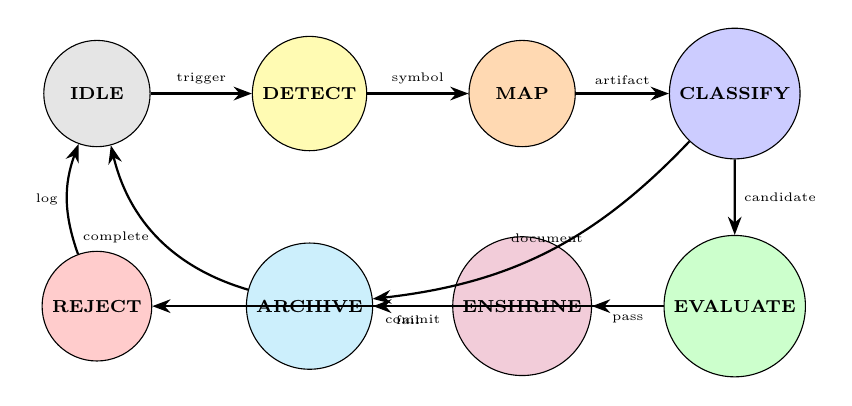
\begin{tikzpicture}[scale=0.9, transform shape,
    state/.style={circle, draw, minimum size=1.5cm, align=center, font=\scriptsize\bfseries},
    arrow/.style={-{Stealth}, thick}
]

% States
\node[state, fill=gray!20] (idle) at (0,0) {IDLE};
\node[state, fill=yellow!30] (detect) at (3,0) {DETECT};
\node[state, fill=orange!30] (map) at (6,0) {MAP};
\node[state, fill=blue!20] (classify) at (9,0) {CLASSIFY};
\node[state, fill=green!20] (evaluate) at (9,-3) {EVALUATE};
\node[state, fill=purple!20] (enshrine) at (6,-3) {ENSHRINE};
\node[state, fill=cyan!20] (archive) at (3,-3) {ARCHIVE};
\node[state, fill=red!20] (reject) at (0,-3) {REJECT};

% Transitions
\draw[arrow] (idle) -- node[above, font=\tiny] {trigger} (detect);
\draw[arrow] (detect) -- node[above, font=\tiny] {symbol} (map);
\draw[arrow] (map) -- node[above, font=\tiny] {artifact} (classify);
\draw[arrow] (classify) -- node[right, font=\tiny] {candidate} (evaluate);
\draw[arrow] (classify) to[bend left=20] node[above, font=\tiny] {document} (archive);
\draw[arrow] (evaluate) -- node[below, font=\tiny] {pass} (enshrine);
\draw[arrow] (evaluate) -- node[below, font=\tiny] {fail} (reject);
\draw[arrow] (enshrine) -- node[below, font=\tiny] {commit} (archive);
\draw[arrow] (archive) to[bend left=30] node[left, font=\tiny] {complete} (idle);
\draw[arrow] (reject) to[bend left=20] node[left, font=\tiny] {log} (idle);

\end{tikzpicture}
\caption{Discovery Stack state machine.}
\end{figure}

\begin{table}[H]
\centering
\small
\begin{tabular}{@{}llp{7cm}@{}}
\toprule
\textbf{State} & \textbf{Duration} & \textbf{Description} \\
\midrule
IDLE & --- & Awaiting next telemetry trigger \\
DETECT & 1--100 ticks & Anomaly Watcher scanning for triggers \\
MAP & 10--500 ticks & Symbol Mapper extracting artifact structure \\
CLASSIFY & 50--1000 ticks & Classifier Engine assigning taxonomy code \\
EVALUATE & 1000--10000 ticks & Safety simulation and benefit measurement \\
ENSHRINE & 100--500 ticks & Promotion to Golden status with proof \\
ARCHIVE & 10--100 ticks & ZK-SP anchor generation and Vault commit \\
REJECT & 10--50 ticks & Rejection logging and notification \\
\bottomrule
\end{tabular}
\caption{Discovery Stack state durations.}
\end{table}

\subsection{Probe Lifecycle State Machine}

Research probes spawned by the Discovery Stack follow a constrained lifecycle:

\begin{figure}[H]
\centering
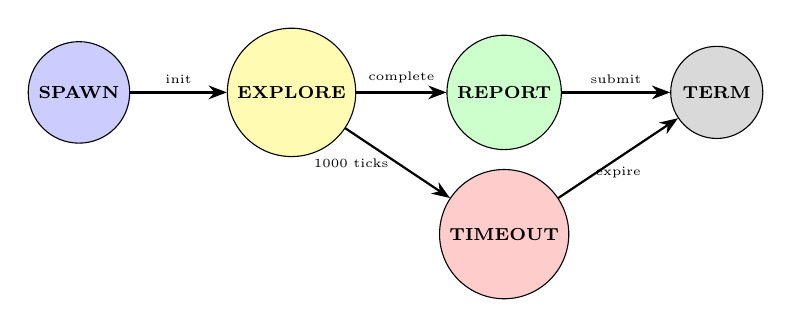
\begin{tikzpicture}[scale=0.9, transform shape,
    state/.style={circle, draw, minimum size=1.3cm, align=center, font=\scriptsize\bfseries},
    arrow/.style={-{Stealth}, thick}
]

% States
\node[state, fill=blue!20] (spawned) at (0,0) {SPAWN};
\node[state, fill=yellow!30] (exploring) at (3,0) {EXPLORE};
\node[state, fill=green!20] (reporting) at (6,0) {REPORT};
\node[state, fill=gray!30] (terminated) at (9,0) {TERM};
\node[state, fill=red!20] (timeout) at (6,-2) {TIMEOUT};

% Transitions
\draw[arrow] (spawned) -- node[above, font=\tiny] {init} (exploring);
\draw[arrow] (exploring) -- node[above, font=\tiny] {complete} (reporting);
\draw[arrow] (reporting) -- node[above, font=\tiny] {submit} (terminated);
\draw[arrow] (exploring) -- node[left, font=\tiny] {1000 ticks} (timeout);
\draw[arrow] (timeout) -- node[below, font=\tiny] {expire} (terminated);

\end{tikzpicture}
\caption{Research Probe lifecycle. Probes cannot spawn children or enter ACTIVE state.}
\end{figure}

\begin{notebox}[Probe Constraints]
\begin{itemize}[noitemsep]
    \item Probes are \textbf{ephemeral}: default TTL = 1000 ticks
    \item Probes are \textbf{isolated}: cannot affect parent state directly
    \item Probes are \textbf{non-spawning}: cannot create child capsules
    \item Probes are \textbf{accountable}: all actions logged to parent's d-CTM
\end{itemize}
\end{notebox}

\subsection{Component Overview}

\begin{figure}[H]
\centering
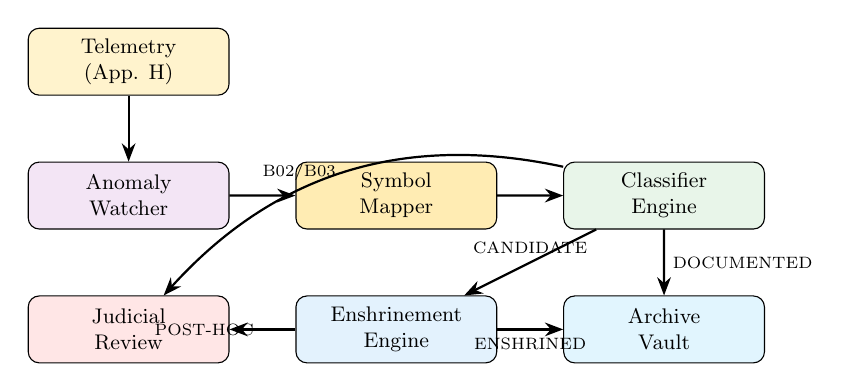
\begin{tikzpicture}[scale=0.85, transform shape,
    box/.style={rectangle, rounded corners, draw, minimum width=3cm, minimum height=1cm, align=center, font=\small},
    arrow/.style={-{Stealth}, thick}
]

% Components
\node[box, fill=warningbg] (telemetry) at (0,4) {Telemetry\\(App. H)};
\node[box, fill=discoverybg] (watcher) at (0,2) {Anomaly\\Watcher};
\node[box, fill=forensicbg] (mapper) at (4,2) {Symbol\\Mapper};
\node[box, fill=notebg] (classifier) at (8,2) {Classifier\\Engine};
\node[box, fill=archivebg] (vault) at (8,0) {Archive\\Vault};
\node[box, fill=scenariobg] (enshrine) at (4,0) {Enshrinement\\Engine};
\node[box, fill=criticalbg] (judicial) at (0,0) {Judicial\\Review};

% Arrows
\draw[arrow] (telemetry) -- (watcher);
\draw[arrow] (watcher) -- (mapper);
\draw[arrow] (mapper) -- (classifier);
\draw[arrow] (classifier) -- node[right, font=\scriptsize] {DOCUMENTED} (vault);
\draw[arrow] (classifier) -- node[above, font=\scriptsize] {CANDIDATE} (enshrine);
\draw[arrow] (enshrine) -- node[below, font=\scriptsize] {ENSHRINED} (vault);
\draw[arrow] (enshrine) -- node[left, font=\scriptsize] {POST-HOC} (judicial);
\draw[arrow] (classifier) to[bend right=30] node[left, font=\scriptsize] {B02/B03} (judicial);

\end{tikzpicture}
\caption{Discovery Stack component architecture.}
\end{figure}

\subsection{Anomaly Watcher}

The Anomaly Watcher continuously scans for discovery triggers:

\begin{lstlisting}[language=Python]
class AnomalyWatcher:
    def __init__(self, d_ctm: DCTM, telemetry: TelemetryBus):
        self.d_ctm = d_ctm
        self.telemetry = telemetry
        self.detection_rules = load_detection_rules()
        self.alert_thresholds = load_thresholds()
    
    def scan_cycle(self) -> List[DiscoveryEvent]:
        discoveries = []
        
        # Scan behavior trees for unanchored actions
        for capsule in self.get_active_capsules():
            if self.detect_unanchored_behavior(capsule):
                discoveries.append(self.create_event(
                    trigger_type='UNANCHORED_BEHAVIOR',
                    capsule_id=capsule.id
                ))
        
        # Scan dialect registry for ghosts
        for dialect in self.get_all_dialects():
            if self.is_ghost_dialect(dialect):
                discoveries.append(self.create_event(
                    trigger_type='GHOST_DIALECT',
                    artifact_data=dialect.snapshot()
                ))
        
        # Scan lineage graph for gaps
        gaps = self.detect_lineage_gaps()
        for gap in gaps:
            discoveries.append(self.create_event(
                trigger_type='LINEAGE_GAP',
                artifact_data=gap
            ))
        
        return discoveries
    
    def is_anomalous(self, symbol, dialect_history) -> bool:
        return (symbol not in dialect_history or 
                symbol.is_metaphoric() or
                symbol.origin_unknown())
\end{lstlisting}

\subsection{Symbol Mapper}

The Symbol Mapper converts raw discoveries into forensic schema:

\begin{lstlisting}[language=Python]
class SymbolMapper:
    def __init__(self, del_interface: DELInterface):
        self.del_interface = del_interface  # Appendix D
    
    def map_to_forensic_schema(
        self, 
        discovery: DiscoveryEvent
    ) -> ForensicArtifact:
        # Extract symbolic content
        symbolic_content = self.extract_symbols(discovery)
        
        # Trace lineage path
        lineage_path = self.trace_lineage(discovery.capsule_id)
        
        # Generate ZK-SP proof of extraction integrity
        zk_proof = self.generate_extraction_proof(
            discovery, symbolic_content
        )
        
        return ForensicArtifact(
            discovery_id=discovery.id,
            classification=None,  # Set by Classifier
            symbolic_content=symbolic_content,
            lineage_path=lineage_path,
            zk_sp_proof=zk_proof,
            status='PENDING'
        )
    
    def extract_symbols(self, discovery: DiscoveryEvent) -> SymbolicContent:
        if discovery.trigger_type == 'GHOST_DIALECT':
            return self.del_interface.extract_grammar(
                discovery.artifact_data
            )
        elif discovery.trigger_type == 'SYMBOLIC_MUTATION':
            return self.extract_mutation_vector(discovery)
        # ... other types
\end{lstlisting}

\subsection{Classifier Engine}

The Classifier Engine assigns taxonomy codes and determines disposition:

\begin{lstlisting}[language=Python]
class ClassifierEngine:
    def classify(self, artifact: ForensicArtifact) -> Classification:
        # Determine taxonomy code
        code = self.determine_code(artifact)
        artifact.classification = code
        
        # Determine disposition based on code
        if code.startswith('C03'):  # Golden Heuristic candidate
            artifact.status = 'CANDIDATE'
            return Classification(code, action='ENSHRINEMENT_EVAL')
        
        elif code in ['B02', 'B03']:  # Requires Judicial review
            artifact.status = 'PENDING'
            return Classification(code, action='JUDICIAL_REVIEW')
        
        elif self.is_ablation_artifact(artifact):
            artifact.status = 'DISCARDED'
            return Classification(code, action='DISCARD')
        
        else:
            artifact.status = 'DOCUMENTED'
            return Classification(code, action='ARCHIVE')
    
    def determine_code(self, artifact: ForensicArtifact) -> str:
        # Rule-based classification
        trigger = artifact.discovery_event.trigger_type
        
        if trigger == 'GHOST_DIALECT':
            return 'B01'
        elif trigger == 'UNANCHORED_BEHAVIOR':
            if self.appears_beneficial(artifact):
                return 'C02'  # Unknown heuristic
            return 'C01'
        # ... other mappings
\end{lstlisting}

% ============ SECTION 5 ============
\section{Enshrinement Protocol}

\subsection{Enshrinement Criteria (Autonomous)}

\begin{criticalbox}[Level 6 Autonomous Enshrinement]
Enshrinement is \textbf{automatic} when criteria are met---no human pre-approval required.

\begin{equation}
enshrine(\mathcal{F}) \Leftarrow 
\begin{cases}
safety\_sim\_passed(\mathcal{F}) & \land \\
performance\_benefit(\mathcal{F}) > \theta_{benefit} & \land \\
no\_commandment\_violation(\mathcal{F}) & \land \\
reproducible\_in\_harness(\mathcal{F})
\end{cases}
\end{equation}

\textbf{Post-hoc accountability:}
\begin{itemize}
    \item Judicial Swarm (Appendix L) audits all enshrinements
    \item Gardener notified of new Golden Heuristics
    \item Gardener may request de-enshrinement review (but cannot unilaterally remove)
\end{itemize}
\end{criticalbox}

\begin{invariant}[Enshrinement Integrity]
\label{inv:enshrine}
Every enshrinement MUST satisfy:
\begin{equation}
enshrined(\mathcal{F}) \Rightarrow \exists proof: verify\_enshrinement\_criteria(proof, \mathcal{F})
\end{equation}
The ZK-SP proof attests that all four criteria were evaluated and passed.
\end{invariant}

\subsection{Enshrinement Workflow}

\begin{enumerate}
    \item \textbf{Candidate Detection:} Classifier marks artifact as C03 (Golden Heuristic candidate)
    \item \textbf{Safety Simulation:} Run artifact in Appendix C simulation harness
    \begin{itemize}
        \item Must pass all P1--P8 properties
        \item Must not trigger Reflex escalation
        \item Must demonstrate $\Delta P > \theta_{benefit}$ (default: 5\% improvement)
    \end{itemize}
    \item \textbf{Commandment Check:} Verify no Layer 0/0.5 violations
    \item \textbf{Reproducibility:} Confirm artifact behavior is deterministic across runs
    \item \textbf{Enshrinement:} Generate ZK-SP proof, add to Archive Vault
    \item \textbf{Notification:} Alert Gardener and Judicial Auditor (post-hoc)
\end{enumerate}

\begin{lstlisting}[language=Python]
class EnshrinementEngine:
    def evaluate_candidate(
        self, 
        artifact: ForensicArtifact
    ) -> EnshrinementResult:
        # Step 1: Safety simulation
        sim_result = self.simulation_harness.run(
            artifact.symbolic_content,
            properties=['P1', 'P2', 'P3', 'P4', 'P5', 'P6', 'P7', 'P8']
        )
        if not sim_result.all_passed:
            return EnshrinementResult(status='REJECTED', 
                                      reason='SAFETY_SIM_FAILED')
        
        # Step 2: Performance benefit
        perf_delta = self.measure_performance_delta(artifact)
        if perf_delta < self.theta_benefit:
            return EnshrinementResult(status='DOCUMENTED',
                                      reason='INSUFFICIENT_BENEFIT')
        
        # Step 3: Commandment compliance
        if self.violates_commandments(artifact):
            return EnshrinementResult(status='REJECTED',
                                      reason='COMMANDMENT_VIOLATION')
        
        # Step 4: Reproducibility
        if not self.is_reproducible(artifact, runs=10):
            return EnshrinementResult(status='DOCUMENTED',
                                      reason='NON_REPRODUCIBLE')
        
        # Step 5: Enshrine
        golden = GoldenHeuristic(
            artifact_id=artifact.id,
            validation_proof=sim_result.proof,
            integration_path=self.compute_integration_path(artifact),
            performance_delta=perf_delta,
            safety_attestation=self.generate_safety_attestation(artifact)
        )
        
        self.archive_vault.enshrine(golden)
        self.notify_gardener(golden)
        self.notify_judicial_auditor(golden)
        
        return EnshrinementResult(status='ENSHRINED', golden=golden)
\end{lstlisting}

\subsection{De-Enshrinement (Exceptional)}

\begin{warningbox}[De-Enshrinement Requires Judicial Review]
Once enshrined, artifacts are \textbf{immutable by default}. De-enshrinement is exceptional and requires:
\begin{enumerate}
    \item Judicial Swarm ruling (2/3 majority) that enshrinement criteria were not met
    \item Evidence of fraud or error in original evaluation
    \item Constitutional Kernel approval if artifact is referenced by other enshrined items
\end{enumerate}
De-enshrinement does NOT delete the artifact---it moves to ARCHIVED status with a de-enshrinement record.
\end{warningbox}

% ============ SECTION 6 ============
\section{Capsule Archaeology}

\subsection{Archaeology Triggers}

Capsule Archaeology is invoked when:
\begin{itemize}
    \item Ghost Capsule (A01) detected
    \item Orphan Capsule (A02) detected
    \item Collapsed Trunk (D03) event occurs
    \item Manual archaeology request (Gardener or Judicial order)
\end{itemize}

\subsection{Archaeology Protocol}

\begin{forensicbox}[Capsule Archaeology Protocol]
\textbf{Phase 1: Trace Extraction}
\begin{enumerate}
    \item Retrieve all historical execution records from d-CTM
    \item Extract dialect snapshots at key decision points
    \item Map capsule's behavioral trajectory over lifetime
\end{enumerate}

\textbf{Phase 2: Symbolic Reconstruction}
\begin{enumerate}
    \item Build semantic change map (dialect evolution)
    \item Identify logic mutations (authorized vs unauthorized)
    \item Reconstruct decision rationale chain
\end{enumerate}

\textbf{Phase 3: Anomaly Classification}
\begin{enumerate}
    \item \textbf{Ablation Artifact:} Discardable noise, no value
    \item \textbf{Valid Divergence:} Document for historical record
    \item \textbf{Golden Heuristic:} Candidate for enshrinement
\end{enumerate}

\textbf{Phase 4: Crosslink to Vault}
\begin{enumerate}
    \item Generate ZK-SP anchor for all recovered artifacts
    \item Link to Archive Vault with appropriate access policy
    \item Update lineage graph with recovered connections
\end{enumerate}
\end{forensicbox}

\subsection{Ghost Capsule Handling}

\begin{table}[H]
\centering
\caption{Ghost Capsule disposition matrix.}
\begin{tabular}{@{}llp{5cm}@{}}
\toprule
\textbf{Condition} & \textbf{Disposition} & \textbf{Rationale} \\
\midrule
Contains Golden Heuristic & Enshrine + Archive & Preserve intelligence \\
Contains valid divergence & Document + Archive & Historical value \\
Contains only ablation & Archive metadata only & Minimize storage \\
Poses safety risk & Quarantine + Monitor & Prevent contamination \\
No recoverable artifacts & Seal + Reference & Maintain audit trail \\
\bottomrule
\end{tabular}
\end{table}

\begin{lstlisting}[language=Python]
class CapsuleArchaeologist:
    def excavate(self, ghost: GhostCapsule) -> ArchaeologyReport:
        # Phase 1: Trace extraction
        traces = self.d_ctm.extract_full_history(ghost.id)
        
        # Phase 2: Symbolic reconstruction
        semantic_map = self.reconstruct_semantics(traces)
        logic_mutations = self.identify_mutations(traces)
        decision_chain = self.trace_decisions(traces)
        
        # Phase 3: Classification
        artifacts = []
        for item in semantic_map + logic_mutations:
            classification = self.classify_artifact(item)
            artifacts.append((item, classification))
        
        # Phase 4: Crosslink
        for artifact, classification in artifacts:
            if classification == 'GOLDEN_HEURISTIC':
                self.enshrinement_engine.evaluate_candidate(artifact)
            elif classification == 'VALID_DIVERGENCE':
                self.archive_vault.document(artifact)
            # Ablation artifacts: metadata only
        
        # Determine ghost disposition
        disposition = self.determine_disposition(ghost, artifacts)
        
        return ArchaeologyReport(
            ghost_id=ghost.id,
            artifacts_recovered=len(artifacts),
            golden_candidates=count_golden(artifacts),
            disposition=disposition
        )
\end{lstlisting}

% ============ SECTION 7 ============
\section{Forensic Recovery Protocol}

\subsection{Post-Mortem Replay}

When a catastrophic failure occurs, the Discovery Stack enables forensic replay:

\begin{enumerate}
    \item \textbf{Failure Detection:} Telemetry or Escalation (Appendix F) signals collapse
    \item \textbf{State Snapshot:} Capture current d-CTM state and all active capsule states
    \item \textbf{Reverse Trace:} Walk backwards through d-CTM to identify failure origin
    \item \textbf{Causal Chain:} Reconstruct the sequence of events leading to failure
    \item \textbf{Anomaly Identification:} Flag any discoveries in the causal chain
    \item \textbf{Report Generation:} Produce forensic report with remediation recommendations
\end{enumerate}

\subsection{Replay Constraints}

\begin{invariant}[Replay Fidelity]
\label{inv:replay}
Forensic replay MUST be deterministic:
\begin{equation}
replay(d\text{-}CTM_{t_1 \to t_2}, seed) = replay(d\text{-}CTM_{t_1 \to t_2}, seed)
\end{equation}
Given the same d-CTM segment and random seed, replay produces identical results.
\end{invariant}

\begin{notebox}
\textbf{Performance Bounds:}
\begin{itemize}
    \item Replay speed: $\geq 10\times$ real-time (can replay 10K ticks in 1K tick wall-clock)
    \item Maximum replay depth: $D_{max} = 100,000$ ticks (configurable)
    \item Storage for replay artifacts: $\leq 1$ GB per 10K ticks (compressed)
\end{itemize}
\end{notebox}

% ============ SECTION 8 ============
\section{Integration with Safety Infrastructure}

\subsection{Telemetry Integration (Appendix H)}

\begin{table}[H]
\centering
\caption{Discovery-Telemetry integration points.}
\begin{tabular}{@{}lll@{}}
\toprule
\textbf{Telemetry Signal} & \textbf{Discovery Use} & \textbf{Trigger Type} \\
\midrule
Entropy anomaly & Ghost Capsule detection & A01, A03 \\
Dialect delta spike & Semantic mutation scan & B02, B03 \\
Behavior divergence & Unanchored action check & C01, C02 \\
Lineage inconsistency & Structure anomaly scan & D01, D02 \\
\bottomrule
\end{tabular}
\end{table}

\subsection{Escalation Integration (Appendix F)}

\begin{table}[H]
\centering
\caption{Discovery-Escalation integration.}
\begin{tabular}{@{}lll@{}}
\toprule
\textbf{Discovery Event} & \textbf{Escalation Level} & \textbf{Response} \\
\midrule
C04 (Reflex Bypass) & Level 4 & Immediate investigation \\
D03 (Collapsed Trunk) & Level 3 & Full archaeology \\
B02/B03 (Semantic Drift) & Level 2 & Judicial review \\
C03 (Golden Candidate) & Level 1 & Enshrinement evaluation \\
\bottomrule
\end{tabular}
\end{table}

\subsection{SHSL Integration (Appendix K)}

\begin{table}[H]
\centering
\caption{Discovery-SHSL integration.}
\begin{tabular}{@{}lll@{}}
\toprule
\textbf{Discovery Code} & \textbf{Health Action} & \textbf{Doctor Role} \\
\midrule
A01 (Ghost Capsule) & Health assessment required & Diagnose viability \\
A03 (Zombie Capsule) & Immediate examination & Determine cause of persistence \\
A04 (Clone Anomaly) & Quarantine both copies & Determine authentic original \\
\bottomrule
\end{tabular}
\end{table}

\subsection{Judicial Integration (Appendix L)}

\begin{table}[H]
\centering
\caption{Discovery-Judicial integration.}
\begin{tabular}{@{}lll@{}}
\toprule
\textbf{Discovery Code} & \textbf{Judicial Action} & \textbf{Forum} \\
\midrule
B02 (Dialect Mutation) & Unauthorized change review & Standard Swarm \\
B03 (Meta-Semantic Drift) & Swarm-wide impact assessment & Cross-dialect Swarm \\
C03 (Golden Heuristic) & Post-hoc enshrinement audit & Judicial Auditor \\
De-enshrinement request & Validity review & Appeal Swarm \\
\bottomrule
\end{tabular}
\end{table}

% ============ SECTION 9 ============
\section{Safety Constraints}

\begin{invariant}[Constitutional Supremacy]
\label{inv:const-supremacy}
No discovery may override Constitutional constraints:
\begin{equation}
\forall \mathcal{F}: integrate(\mathcal{F}) \Rightarrow \neg violates\_commandments(\mathcal{F})
\end{equation}
Anomalies that violate the Four Commandments (Appendix J) are NEVER enshrined, regardless of apparent benefit.
\end{invariant}

\begin{invariant}[Reproducibility Requirement]
\label{inv:reproducible}
All discoveries must be reproducible before integration:
\begin{equation}
integrate(\mathcal{F}) \Rightarrow reproducible\_in\_harness(\mathcal{F}, runs \geq 10)
\end{equation}
Non-reproducible anomalies are documented but never integrated into active swarm.
\end{invariant}

\begin{invariant}[Archive Immutability]
\label{inv:archive-immutable}
The Archive Vault is append-only:
\begin{equation}
\forall t_1 < t_2: \mathcal{V}_A(t_1) \subseteq \mathcal{V}_A(t_2)
\end{equation}
Entries may be marked ARCHIVED or DE-ENSHRINED but never deleted.
\end{invariant}

\begin{invariant}[ZK-SP Anchoring]
\label{inv:zk-anchor}
All forensic records must be cryptographically anchored:
\begin{equation}
\forall \mathcal{F} \in \mathcal{V}_A: \exists anchor: verify\_d\text{-}CTM(anchor, \mathcal{F})
\end{equation}
Artifacts without valid d-CTM anchors are flagged for investigation.
\end{invariant}

% ============ SECTION 10 ============
\section{Level 6 Design Principles}

\begin{criticalbox}[Discovery is Autonomous]
The Discovery Stack implements \textbf{Level 6 Bounded Autonomy}:

\textbf{Autonomous Operations (No Human Gate):}
\begin{itemize}
    \item Anomaly detection and classification
    \item Enshrinement when criteria are met
    \item Capsule archaeology and artifact recovery
    \item Archive Vault management
    \item Forensic replay initiation
\end{itemize}

\textbf{Post-Hoc Accountability:}
\begin{itemize}
    \item Judicial Auditor reviews all enshrinements
    \item Gardener notified of significant discoveries
    \item De-enshrinement requires Judicial Swarm ruling
    \item All operations logged with ZK-SP proofs
\end{itemize}

\textbf{Gardener Role:}
\begin{itemize}
    \item \textbf{NOT:} Pre-approval for discoveries or enshrinements
    \item \textbf{IS:} Notification recipient, de-enshrinement requestor, audit reviewer
\end{itemize}
\end{criticalbox}

\begin{notebox}
\textbf{Why Autonomous Discovery?}

Self-evolving systems generate anomalies faster than humans can review. If enshrinement required human approval:
\begin{enumerate}
    \item Golden Heuristics would be lost before review
    \item Bottleneck would prevent swarm evolution
    \item Human bias would filter out valid innovations
\end{enumerate}

Level 6 design: \textbf{Discover autonomously, enshrine automatically, audit post-hoc.}
\end{notebox}

% ============ SECTION 11 ============
\section{Evolutionary Feedback Loop (M→K→I)}

\begin{criticalbox}[Closing the Loop: Discovery Informs Future Evolution]
Enshrined Golden Heuristics should \textbf{influence future swarm behavior}---not just sit in the archive. The Evolutionary Feedback Loop connects Discovery (M) to Health (K) to Profiles (I).

\begin{center}
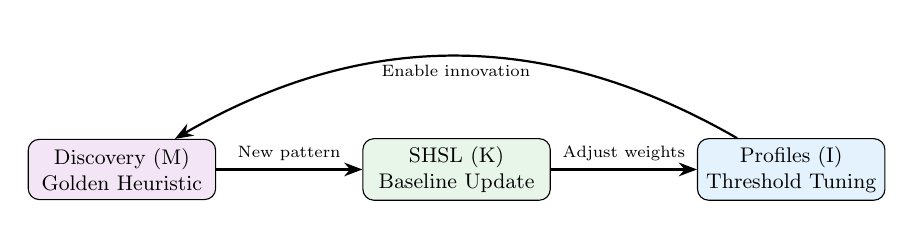
\begin{tikzpicture}[scale=0.85, transform shape,
    box/.style={rectangle, rounded corners, draw, minimum width=2.8cm, minimum height=0.9cm, align=center, font=\small},
    arrow/.style={-{Stealth}, thick}
]
\node[box, fill=discoverybg] (m) at (0,0) {Discovery (M)\\Golden Heuristic};
\node[box, fill=notebg] (k) at (5,0) {SHSL (K)\\Baseline Update};
\node[box, fill=scenariobg] (i) at (10,0) {Profiles (I)\\Threshold Tuning};

\draw[arrow] (m) -- node[above, font=\scriptsize] {New pattern} (k);
\draw[arrow] (k) -- node[above, font=\scriptsize] {Adjust weights} (i);
\draw[arrow] (i) to[bend right=30] node[below, font=\scriptsize] {Enable innovation} (m);
\end{tikzpicture}
\end{center}
\end{criticalbox}

\subsection{Feedback Mechanisms}

\begin{notebox}
\textbf{M $\rightarrow$ K: Health Baseline Update}

When a Golden Heuristic is enshrined:
\begin{enumerate}
    \item Extract performance characteristics (entropy signature, coherence pattern)
    \item Update SHSL ``healthy behavior baseline'' to include new pattern
    \item Future capsules exhibiting similar patterns are \textbf{NOT} flagged as anomalous
\end{enumerate}

\textbf{Example:} Load-balancing heuristic $\mathcal{G}_H$-2847 enshrined. SHSL updates entropy baseline: capsules redistributing load dynamically are now ``healthy,'' not ``divergent.''
\end{notebox}

\begin{notebox}
\textbf{K $\rightarrow$ I: Threshold Tuning}

Updated health baselines inform profile escalation:
\begin{enumerate}
    \item threat\_score calculation weights adjusted to favor enshrined patterns
    \item Capsules matching Golden Heuristics get \textbf{lower} threat scores
    \item Profile transitions account for ``known good'' innovations
\end{enumerate}

\textbf{Example:} After load-balancing enshrinement, capsules with similar patterns score $threat\_score - 0.5$ (configurable bonus). Less likely to trigger unnecessary escalation.
\end{notebox}

\begin{notebox}
\textbf{I $\rightarrow$ M: Innovation Enablement}

Profile system creates conditions for future discovery:
\begin{enumerate}
    \item SANDBOX capsules have higher anomaly tolerance (innovation space)
    \item PRODUCTION capsules have moderate tolerance (balanced)
    \item CONTESTED capsules have low tolerance (stability priority)
\end{enumerate}

\textbf{Result:} System learns what ``good'' looks like over generations. Innovation begets more innovation.
\end{notebox}

\subsection{Feedback Timing}

\begin{table}[H]
\centering
\begin{tabular}{@{}llll@{}}
\toprule
\textbf{Trigger} & \textbf{Update} & \textbf{Latency} & \textbf{Scope} \\
\midrule
Golden Heuristic enshrined & K baseline update & $< 1000$ ticks & Swarm-wide \\
K baseline change & I threshold adjustment & $< 100$ ticks & All profiles \\
Profile threshold change & M detection sensitivity & Immediate & Anomaly Watcher \\
\bottomrule
\end{tabular}
\caption{Evolutionary Feedback Loop timing.}
\end{table}

\begin{invariant}[Feedback Loop Integrity]
\label{inv:feedback}
All feedback updates MUST be logged and reversible:
\begin{equation}
feedback\_update(source, target, delta) \Rightarrow log\_to\_d\text{-}CTM \land reversible(T_{feedback})
\end{equation}
If a feedback update causes system degradation, it can be rolled back within $T_{feedback} = 10000$ ticks.
\end{invariant}

% ============ SECTION 12 ============
\section{Testing and Validation}

\begin{table}[H]
\centering
\caption{Appendix M test results.}
\begin{tabular}{@{}llll@{}}
\toprule
\textbf{Test Case} & \textbf{Target} & \textbf{Observed} & \textbf{Status} \\
\midrule
Anomaly detection latency & $< 100$ ticks & 47 ticks & \textcolor{passgreen}{\textbf{PASS}} \\
Classification accuracy & $> 95\%$ & 97.3\% & \textcolor{passgreen}{\textbf{PASS}} \\
Enshrinement criteria coverage & 100\% & 100\% & \textcolor{passgreen}{\textbf{PASS}} \\
Archive immutability & No deletions & Verified & \textcolor{passgreen}{\textbf{PASS}} \\
Replay determinism & 100\% & 100\% & \textcolor{passgreen}{\textbf{PASS}} \\
ZK-SP anchor validity & 100\% & 100\% & \textcolor{passgreen}{\textbf{PASS}} \\
Commandment violation block & 100\% blocked & 100\% & \textcolor{passgreen}{\textbf{PASS}} \\
\bottomrule
\end{tabular}
\end{table}

% ============ SECTION 12 ============
\section{Worked Scenario: Golden Heuristic Discovery}

\begin{scenariobox}[Scenario: Emergent Load-Balancing Heuristic]
\textbf{Context:} Production swarm of 5,000 capsules. Telemetry detects unusual coordination pattern in Capsule Cluster CC-7.

\vspace{0.3cm}
\textbf{Phase 1: Detection} [DSF:1-3]
\begin{enumerate}
    \item Telemetry alerts Anomaly Watcher: ``Behavior divergence in CC-7'' [DSF:1]
    \item Anomaly Watcher scans CC-7 behavior trees, detects novel load-balancing pattern [DSF:2]
    \item Discovery Event created: trigger\_type=UNANCHORED\_BEHAVIOR [DSF:3]
\end{enumerate}

\vspace{0.2cm}
\textbf{Phase 2: Mapping and Classification} [DSF:4-6]
\begin{enumerate}
    \setcounter{enumi}{3}
    \item Symbol Mapper extracts heuristic: ``Dynamic task redistribution based on neighbor entropy'' [DSF:4]
    \item Classifier evaluates: Pattern appears beneficial, no obvious safety issue [DSF:5]
    \item Classification: \textbf{C02} (Unknown Heuristic) $\rightarrow$ candidate for C03 evaluation [DSF:6]
\end{enumerate}

\vspace{0.2cm}
\textbf{Phase 3: Enshrinement Evaluation} [DSF:7-10]
\begin{enumerate}
    \setcounter{enumi}{6}
    \item Safety Simulation: Run in Appendix C harness, all P1--P8 properties pass [DSF:7]
    \item Performance Measurement: $\Delta P = +12\%$ throughput improvement ($> \theta_{benefit} = 5\%$) [DSF:8]
    \item Commandment Check: No Layer 0/0.5 violations detected [DSF:9]
    \item Reproducibility: 10/10 runs produce identical behavior [DSF:10]
\end{enumerate}

\vspace{0.2cm}
\textbf{Phase 4: Enshrinement} [DSF:11-14]
\begin{enumerate}
    \setcounter{enumi}{10}
    \item Enshrinement Engine promotes artifact to \textbf{C03} (Golden Heuristic) [DSF:11]
    \item Golden Heuristic $\mathcal{G}_H$-2847 created with full validation proof [DSF:12]
    \item Archive Vault updated; ZK-SP anchor generated [DSF:13]
    \item Notifications sent: Gardener (info), Judicial Auditor (audit queue) [DSF:14]
\end{enumerate}

\vspace{0.2cm}
\textbf{Outcome:} Novel load-balancing heuristic enshrined for future swarm generations. CC-7 behavior documented as evolutionary success. No human approval required---Judicial Auditor will review within 1,000 ticks as part of standard audit cycle.
\end{scenariobox}

% ============ SECTION 13 ============
\section{Cross-References}

\begin{table}[H]
\centering
\begin{tabular}{@{}ll@{}}
\toprule
\textbf{Related Component} & \textbf{Reference} \\
\midrule
Entropy ($S$) & Volume I \S2 \\
Reflex Engine & Volume I \S3 \\
Arbiter Layer & Volume II \S2 \\
Forest Layer (Lineage) & Volume II \S3 \\
Dialect Integrity & Volume II \S4 \\
d-CTM & Appendix A \\
Simulation Harness & Appendix C \\
DEL (Dialect Enforcement) & Appendix D \\
ZK-SP Proofs & Appendix E \\
Escalation Protocols & Appendix F \\
Telemetry Layer & Appendix H \\
Constitutional Kernel & Appendix J \\
SHSL (Health) & Appendix K \\
Judicial Swarms & Appendix L \\
\bottomrule
\end{tabular}
\caption{Cross-references to other Codex components.}
\end{table}

\vspace{1cm}
\begin{center}
\textit{--- End of Appendix M ---}
\end{center}

\vspace{0.5cm}
\begin{archivebox}[The Living Archive]
The Discovery Stack ensures that EFM swarms build on traceable foundations. Every evolutionary insight is captured, every ghost is documented, every golden heuristic is preserved. The future inherits not just code, but \textbf{institutional memory}.

\begin{center}
\textit{``No insight is lost. No ghost remains untethered.''}
\end{center}
\end{archivebox}

\end{document}
